\pdfobjcompresslevel=0
\PassOptionsToPackage{table}{xcolor}
\documentclass[final,t,12pt]{beamer}\usepackage[]{graphicx}\usepackage[]{color}
%% maxwidth is the original width if it is less than linewidth
%% otherwise use linewidth (to make sure the graphics do not exceed the margin)
\makeatletter
\def\maxwidth{ %
  \ifdim\Gin@nat@width>\linewidth
    \linewidth
  \else
    \Gin@nat@width
  \fi
}
\makeatother

\definecolor{fgcolor}{rgb}{0.345, 0.345, 0.345}
\newcommand{\hlnum}[1]{\textcolor[rgb]{0.686,0.059,0.569}{#1}}%
\newcommand{\hlstr}[1]{\textcolor[rgb]{0.192,0.494,0.8}{#1}}%
\newcommand{\hlcom}[1]{\textcolor[rgb]{0.678,0.584,0.686}{\textit{#1}}}%
\newcommand{\hlopt}[1]{\textcolor[rgb]{0,0,0}{#1}}%
\newcommand{\hlstd}[1]{\textcolor[rgb]{0.345,0.345,0.345}{#1}}%
\newcommand{\hlkwa}[1]{\textcolor[rgb]{0.161,0.373,0.58}{\textbf{#1}}}%
\newcommand{\hlkwb}[1]{\textcolor[rgb]{0.69,0.353,0.396}{#1}}%
\newcommand{\hlkwc}[1]{\textcolor[rgb]{0.333,0.667,0.333}{#1}}%
\newcommand{\hlkwd}[1]{\textcolor[rgb]{0.737,0.353,0.396}{\textbf{#1}}}%
\let\hlipl\hlkwb

\usepackage{framed}
\makeatletter
\newenvironment{kframe}{%
 \def\at@end@of@kframe{}%
 \ifinner\ifhmode%
  \def\at@end@of@kframe{\end{minipage}}%
  \begin{minipage}{\columnwidth}%
 \fi\fi%
 \def\FrameCommand##1{\hskip\@totalleftmargin \hskip-\fboxsep
 \colorbox{shadecolor}{##1}\hskip-\fboxsep
     % There is no \\@totalrightmargin, so:
     \hskip-\linewidth \hskip-\@totalleftmargin \hskip\columnwidth}%
 \MakeFramed {\advance\hsize-\width
   \@totalleftmargin\z@ \linewidth\hsize
   \@setminipage}}%
 {\par\unskip\endMakeFramed%
 \at@end@of@kframe}
\makeatother

\definecolor{shadecolor}{rgb}{.97, .97, .97}
\definecolor{messagecolor}{rgb}{0, 0, 0}
\definecolor{warningcolor}{rgb}{1, 0, 1}
\definecolor{errorcolor}{rgb}{1, 0, 0}
\newenvironment{knitrout}{}{} % an empty environment to be redefined in TeX

\usepackage{alltt}\usepackage[]{graphicx}\usepackage[]{color}
%% maxwidth is the original width if it is less than linewidth
%% otherwise use linewidth (to make sure the graphics do not exceed the margin)
\makeatletter
\def\maxwidth{ %
  \ifdim\Gin@nat@width>\linewidth
  \linewidth
  \else
  \Gin@nat@width
  \fi
}
\makeatother


\usepackage{alltt}
\usepackage[percent]{overpic}
\usepackage[utf8]{inputenc}
\renewcommand{\sfdefault}{pfu}
\renewcommand{\familydefault}{\sfdefault}
\usepackage{natbib}
\usepackage[most]{tcolorbox}
% \usepackage{sfmath}
\mode<presentation>
{
  % \usetheme{Warsaw}
  % \usetheme{Aachen}
  % \usetheme{Oldi6}
  % \usetheme{I6td}
  \usetheme{I6dv}
  % \usetheme{I6pd}
  % \usetheme{I6pd2}
}
% additional settings
\setbeamerfont{itemize}{size=\normalsize}
\setbeamerfont{itemize/enumerate body}{size=\normalsize}
\setbeamerfont{itemize/enumerate subbody}{size=\normalsize}

% \AtBeginSection[]
% {
% \begin{beamercolorbox}[ht=7ex, wd=0.99\textwidth]{block title}%
%   \usebeamerfont*{group title} 
%   \Large \centering \insertsection
%   \vskip1ex
% \end{beamercolorbox}
% \vspace{-2ex}
% }

%   additional packages
\usepackage{natbib}
\usepackage{amsmath,amsthm, amssymb, latexsym}
\usepackage{exscale}
\usepackage{multirow}
\usepackage{tabularx}
% \boldmath
\usepackage{booktabs, array}
% \usepackage{rotating} %sideways environment
\usepackage[english]{babel}
% \usepackage[latin1]{inputenc}
% height should be 114.3 (45 in), but is temporarily longer
\usepackage[orientation=landscape,size=a1,scale=1.2]{beamerposter}
\listfiles
\graphicspath{{figures/}}
% Display a grid to help align images
% \beamertemplategridbackground[1cm]
\title{\Huge CBASE: Using CALIOP to estimate the base height of cloud fields}
\author{Johannes M\"ulmenst\"adt,\inst{1} Odran Sourdeval,\inst{1} Tristan L'Ecuyer,\inst{2}
  Christoph B\"ohm,\inst{3} Johannes Quaas\inst{1}}
\institute{% (optional, but mostly needed)
  \inst{1}Institute of Meteorology, Universität Leipzig
  \inst{2}University of Wisconsin, Madison
  \inst{3}Institute for Geophysics and Meteorology, Universit\"at zu K\"oln
}

% abbreviations
\usepackage{xspace}
\makeatletter
\DeclareRobustCommand\onedot{\futurelet\@let@token\@onedot}
\def\@onedot{\ifx\@let@token.\else.\null\fi\xspace}
\def\eg{{e.g}\onedot} \def\Eg{{E.g}\onedot}
\def\ie{{i.e}\onedot} \def\Ie{{I.e}\onedot}
\def\cf{{c.f}\onedot} \def\Cf{{C.f}\onedot}
\def\etc{{etc}\onedot}
\def\vs{{vs}\onedot}
\def\wrt{w.r.t\onedot}
\def\dof{d.o.f\onedot}
\def\etal{{et al}\onedot}
\makeatother

\setbeamerfont{group title}{size=\Large,series=\bf}
\newcommand\degree{\ensuremath{{}^\circ}}

\newcommand{\omegaf}{\ensuremath{\omega_{500}}}
\renewcommand\d[2]{\ensuremath{\frac{d#1}{d#2}}}
\newcommand\D[2]{\ensuremath{\frac{D#1}{D#2}}}
\newcommand\dd[2]{\ensuremath{\frac{\partial#1}{\partial#2}}}
\newcommand\ddp[2]{\ensuremath{\partial#1/\partial#2}}
\newcommand\DDP[2]{\ensuremath{D#1/D#2}}
\newcommand\erfaci{ERF$_\text{aci}$}
\newcommand\erfaer{ERF$_\text{aer}$}
\newcommand\cor{\ensuremath{\text{cor}}}
\IfFileExists{upquote.sty}{\usepackage{upquote}}{}
\IfFileExists{upquote.sty}{\usepackage{upquote}}{}
\begin{document}







\begin{frame}[fragile]{}
  \begin{tcolorbox}[tile,%size=fbox,
    nobeforeafter,
    leftright skip = -30pt,
    notitle,
    boxsep=0mm%,
    % width=\textwidth%,boxrule=0pt,
    % colback=blue!20!black,colbacktitle=yellow!50!black]%% ,
    ,colback=white
    %% title=A Raster of Boxes,center title,
    %% ,height fill
    ]
    \begin{tcbitemize}[raster equal height=rows, raster columns = 11
      % ,
      % raster every box/.style={colframe=red!50!black,colback=red!10!white}
      ]
      \tcbitem[blankest,space to=\myspace, raster multicolumn = 3]
      \begin{tcbitemize}[raster columns=1]
        \tcbitem[add to natural height=\myspace, title={Motivation}]
        \begin{itemize}
        \item Unlike cloud top, cloud base is difficult to observe from
          space
        \item However, accurate knowledge of the cloud base height (CBH) --- and thence
          cloud geometric thickness --- would improve estimates of highly uncertain
          variables in the climate system, such as \alert{cloud subadiabaticity}
          and \alert{surface downwelling longwave flux}
        \item A CBH measurement on the A-Train would be particularly
          advantageous because of the possibility of combining CBH with many
          other retrieved cloud properties
        \item In this work, we present the \alert{Cloud Base Altitude Spatial
          Extrapolator (CBASE)}, CALIOP-based estimate of cloud-field base height
        \end{itemize}

        \tcbitem[title={Method}] 
        ~\vfill
          \begin{columns}[T]
            \begin{column}{0.5\linewidth}
              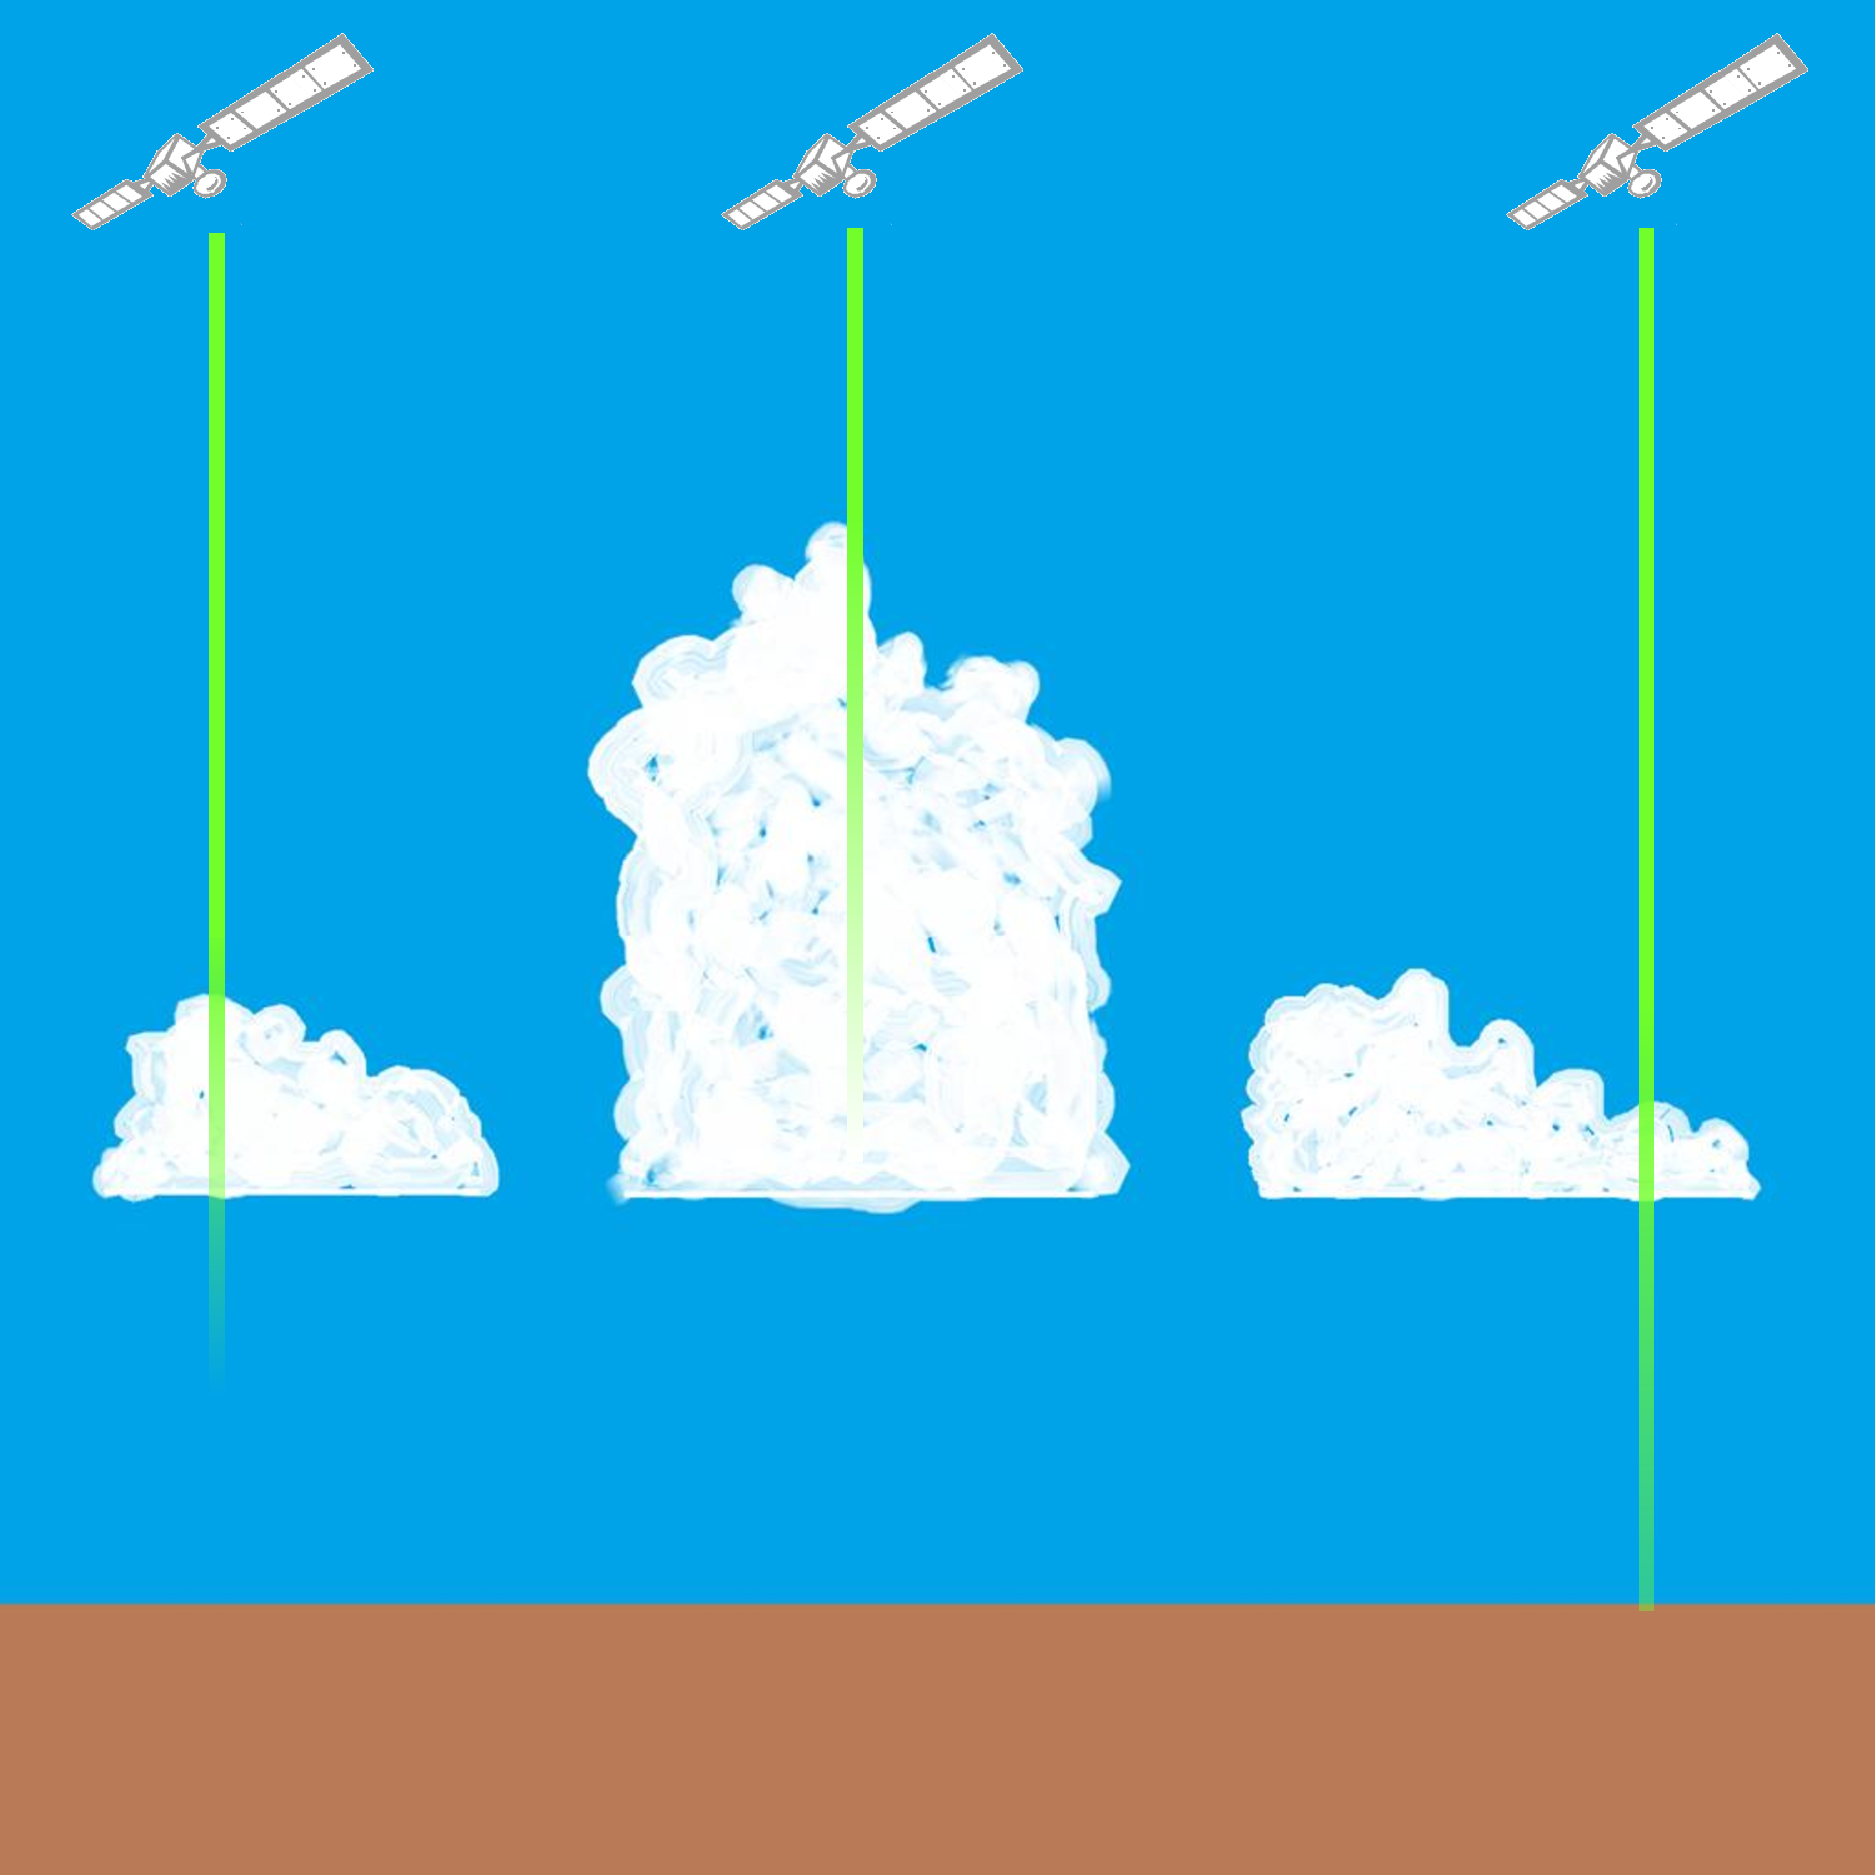
\includegraphics[width=\linewidth,keepaspectratio=true]{CloudFieldCALIOP.pdf}
            \end{column}
            \begin{column}{0.5\linewidth}
              Even though CALIOP attenuates in optically thick ($\tau \gtrsim 5$)
              clouds, the cloud base height of a homogeneous cloud field can be
              inferred from thin clouds or cloud edges that CALIOP can penetrate
            \end{column}
          \end{columns}
        \vfill~

        \tcbitem[title={CBASE algorithm}]
        \begin{enumerate}
        \item We determine the CBH from all CALIOP profiles where the
          surface generates a return, indicating that the lidar is not completely
          attenuated by cloud.  We refer to this as the \textit{local
            CBH} in the sense that it is local to the CALIOP profile.
        \item Using ground-based ceilometer data, we determine quality of cloud base
          height depending on a number of properties of the CALIOP profile.  Assuming
          those properties suffice to determine the quality of the CBH determination, we
          can then predict the quality of a cloud base as a function of those factors.
          The quality metric we use is the root mean square error (RMSE); the category
          RMSE determined from comparison to ceilometer CBH then serves as the predicted
          CBH uncertainty.  In the language of machine learning, we refer to this step
          as \textit{training} the algorithm on the ceilometer data to predict CBH and
          CBH uncertainty.
        \item Based on the predicted quality of each local cloud base, we either reject
          the local cloud base or combine it with other local cloud bases within a
          distance $D_\text{max}$ of the point of interest (POI) to arrive at an 
          estimate of the CBH and its uncertainty at the POI.
        \item Using a \alert{statistically independent validation dataset}, we
          verify that the predicted CBH and its uncertainty are correct.
        \end{enumerate}

      \end{tcbitemize}

      \tcbitem[blankest,space to=\myspace, raster multicolumn = 4]
      \begin{tcbitemize}[raster columns=1]
        \tcbitem[add to natural height=\myspace,
        title={``Ground truth''}]
\begin{knitrout}
\definecolor{shadecolor}{rgb}{0.969, 0.969, 0.969}\color{fgcolor}

{\centering 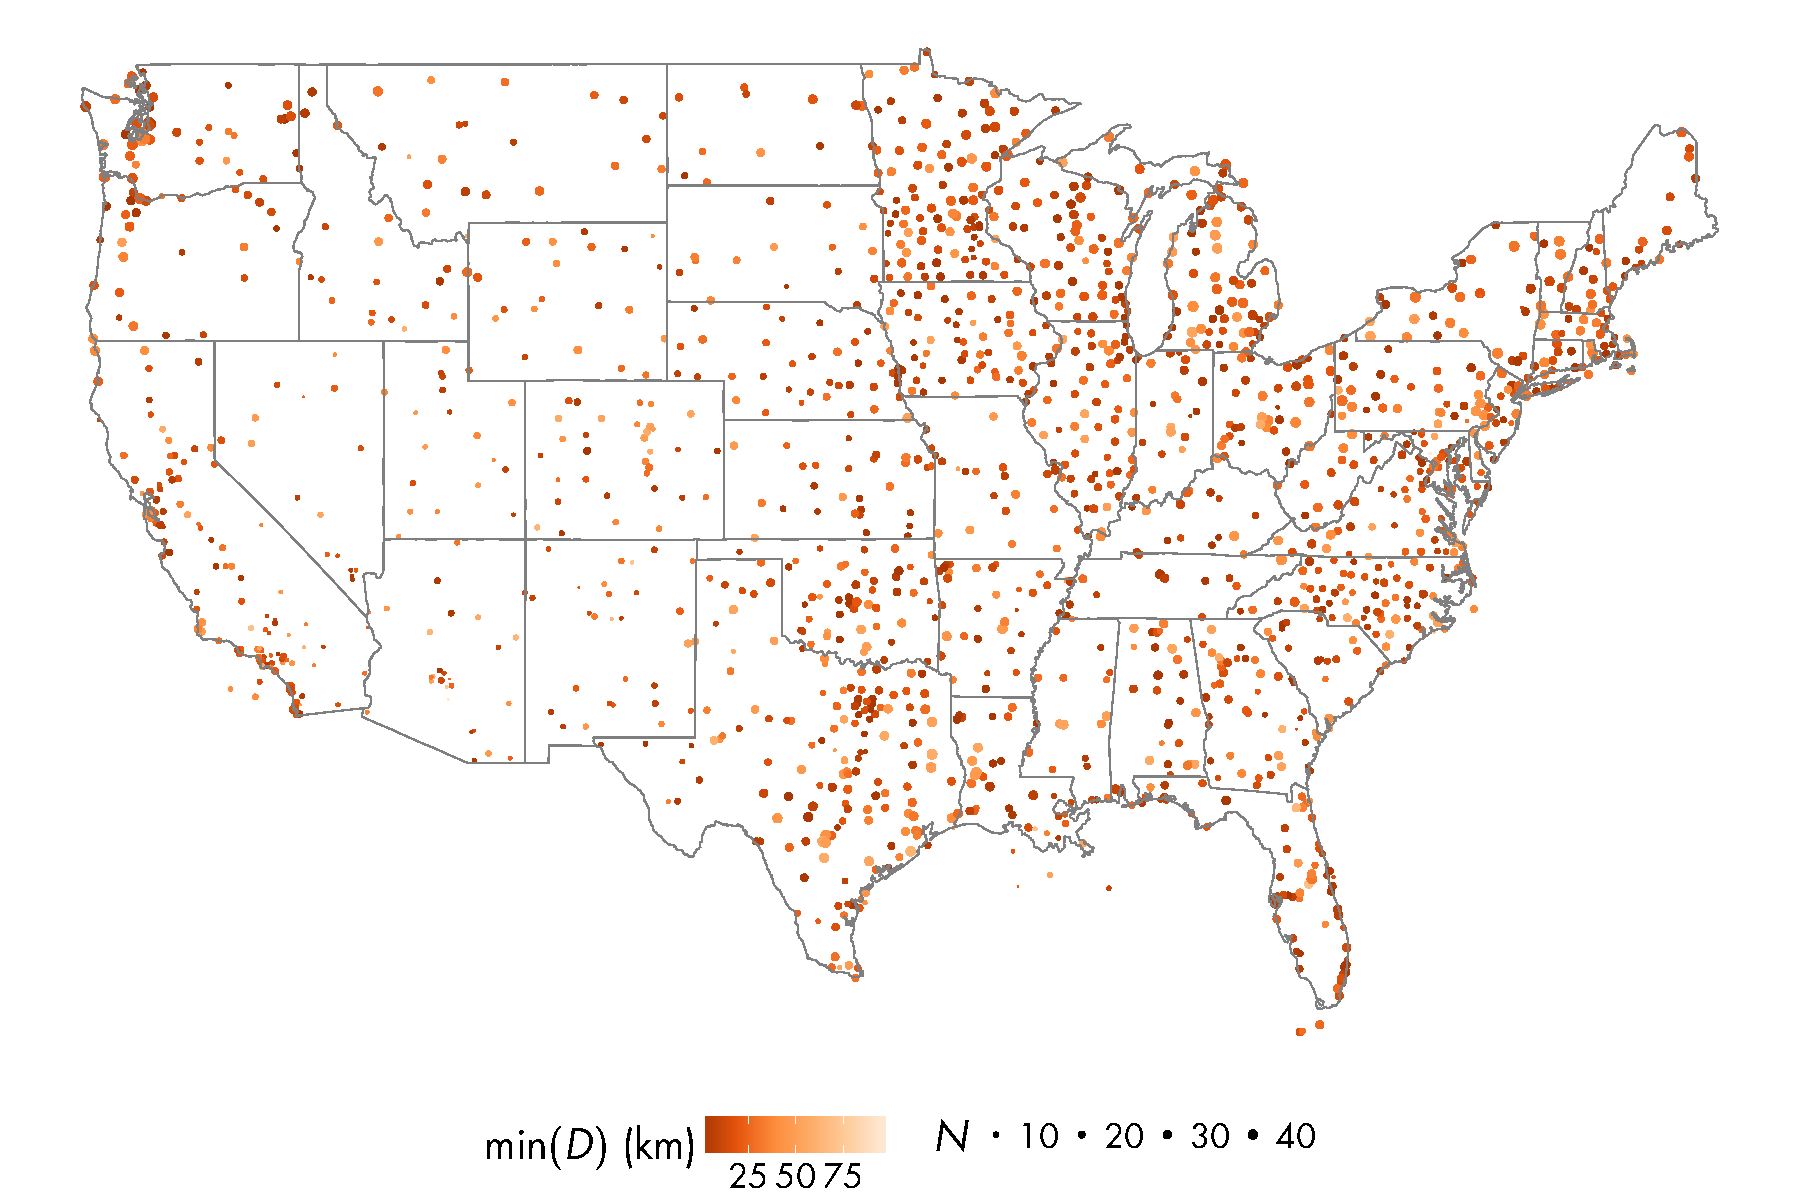
\includegraphics[width=\textwidth]{figure/cfmip-cbase-170926-eval-asos-1} 

}



\end{knitrout}
        Automated Surface Observing System (ASOS) ceilometers are used to train
        (using the year 2008) and validate (using the year 2007) the CBASE
        algorithm

        \tcbitem[title={Validation: How well do we estimate CBH and CBH uncertainty?}] 
        \begin{columns}
          \begin{column}{0.5\linewidth}
\begin{knitrout}
\definecolor{shadecolor}{rgb}{0.969, 0.969, 0.969}\color{fgcolor}

{\centering 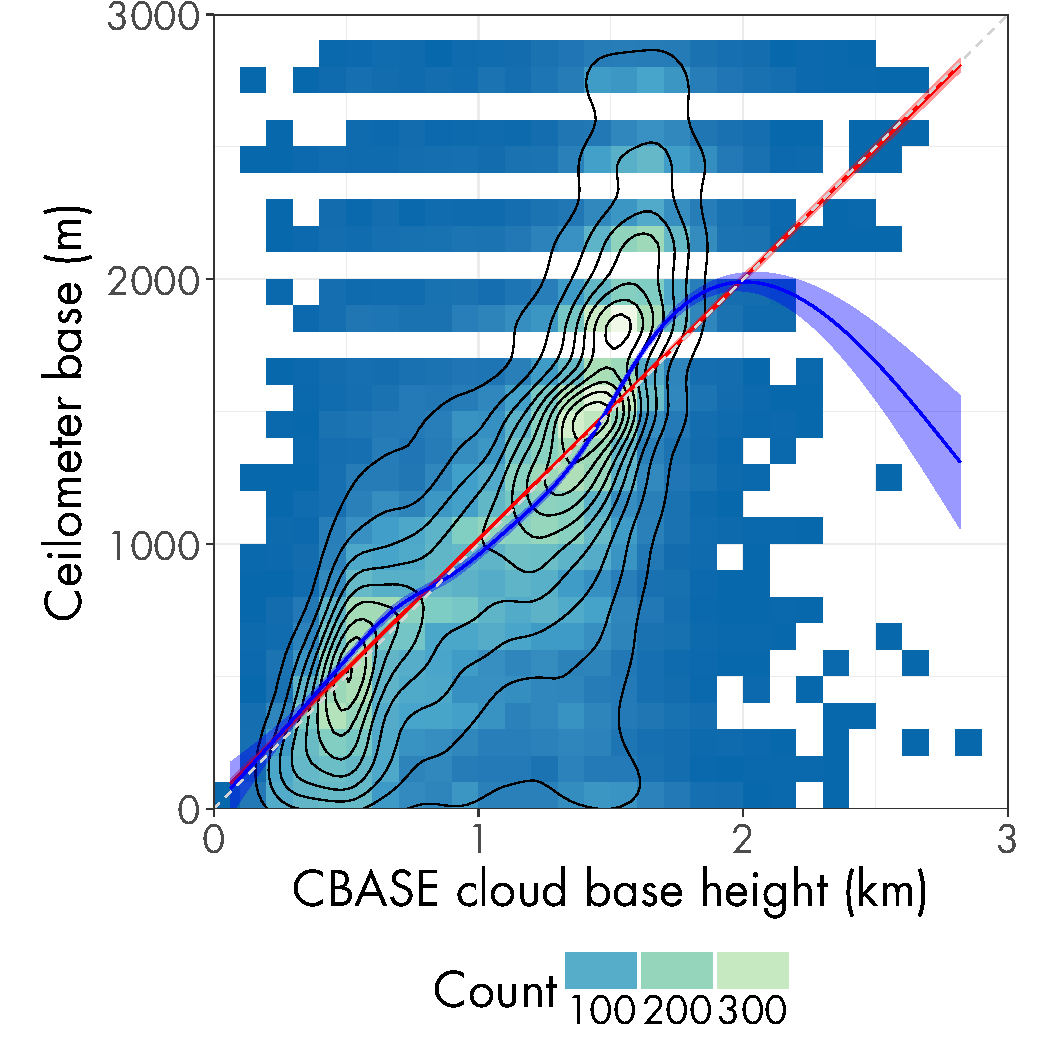
\includegraphics[width=\textwidth]{figure/cfmip-cbase-170926-combo-plot-1} 

}



\end{knitrout}
            {\small \quad Joint histogram of CBASE and ceilometer CBH; 1:1 \quad
              line, linear
              fit, and LOESS fit }
          \end{column}
          \begin{column}{0.5\linewidth}
\begin{knitrout}
\definecolor{shadecolor}{rgb}{0.969, 0.969, 0.969}\color{fgcolor}

{\centering 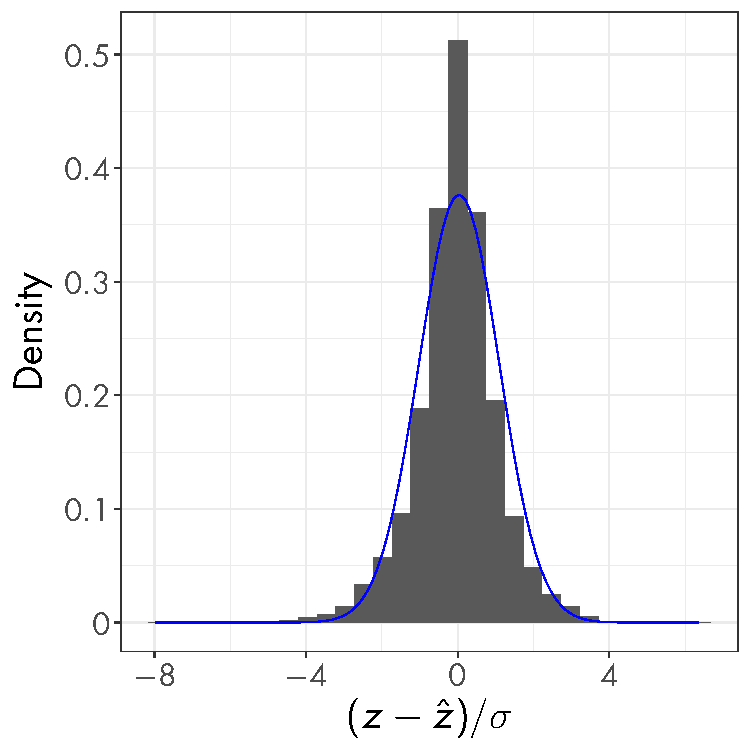
\includegraphics[width=\textwidth]{figure/cfmip-cbase-170926-combo-eval-pull-1} 

}



\end{knitrout}
            
            {\small \quad Cloud base error divided by predicted uncertainty}
          \end{column}
        \end{columns}
        ~\\[24pt] Unbiased CBH and unbiased uncertainty would yield Gaussian with
        zero mean (actual mean: 0.04) and unit standard deviation (actual SD:
        1.06); we
        find \alert{the CBH and its uncertainty to be unbiased to better than
          10\%.}

      \end{tcbitemize}
      
      \tcbitem[blankest,space to=\myspace, raster multicolumn = 4]
      \begin{tcbitemize}[raster columns=1]
        \tcbitem[title={Daytime and nighttime CBH distributions}]


\begin{knitrout}
\definecolor{shadecolor}{rgb}{0.969, 0.969, 0.969}\color{fgcolor}

{\centering 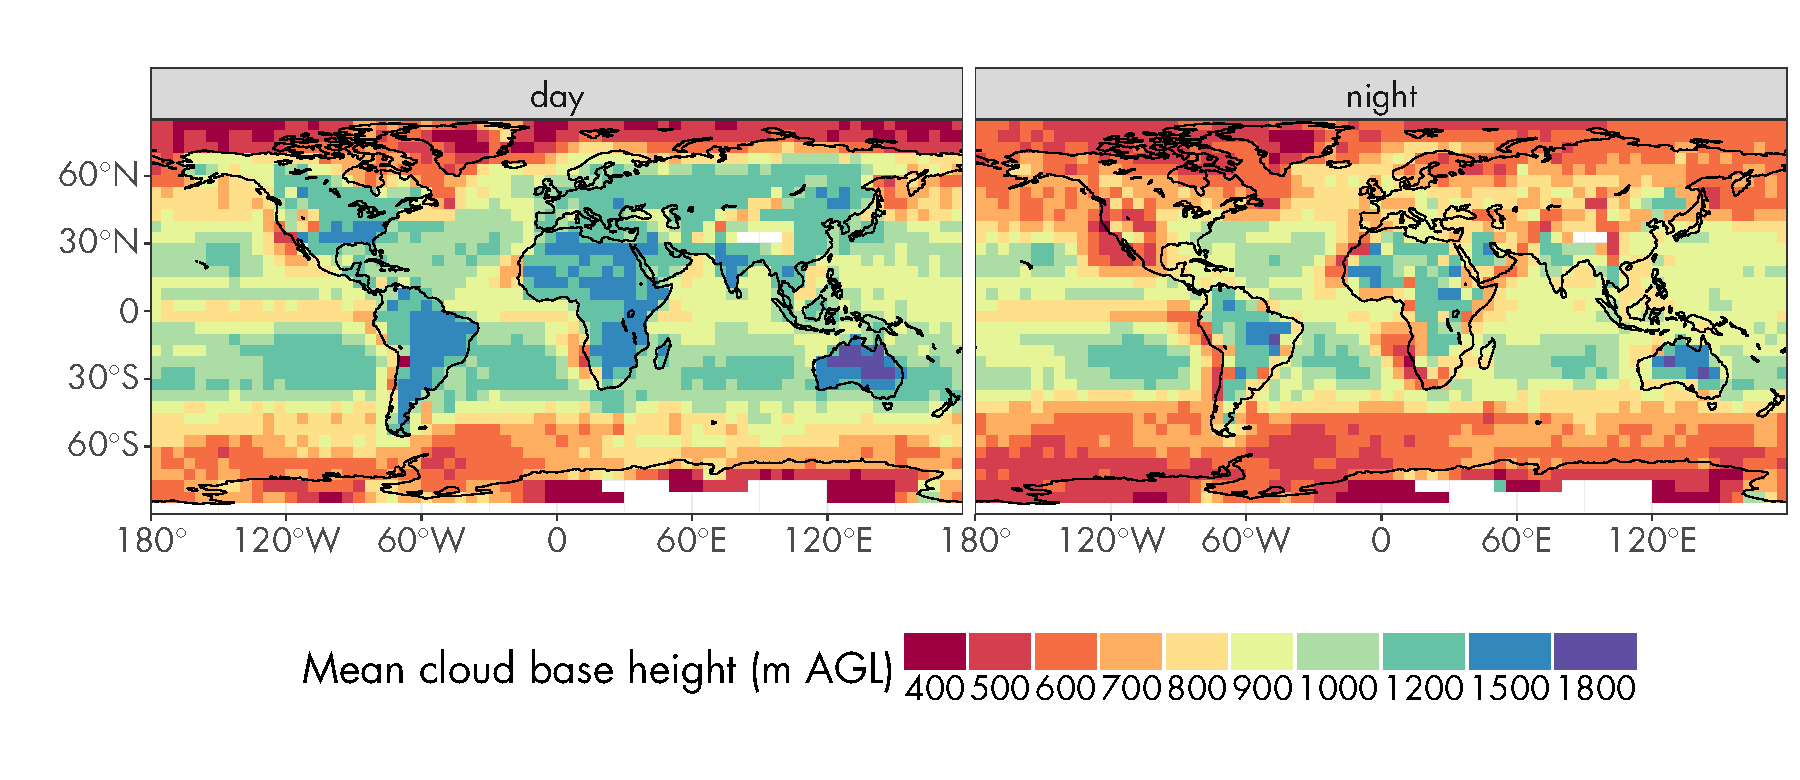
\includegraphics[width=\textwidth]{figure/cfmip-cbase-170926-cbase-base-1} 

}



\end{knitrout}

        \tcbitem[title={CBH uncertainty}]
\begin{knitrout}
\definecolor{shadecolor}{rgb}{0.969, 0.969, 0.969}\color{fgcolor}

{\centering 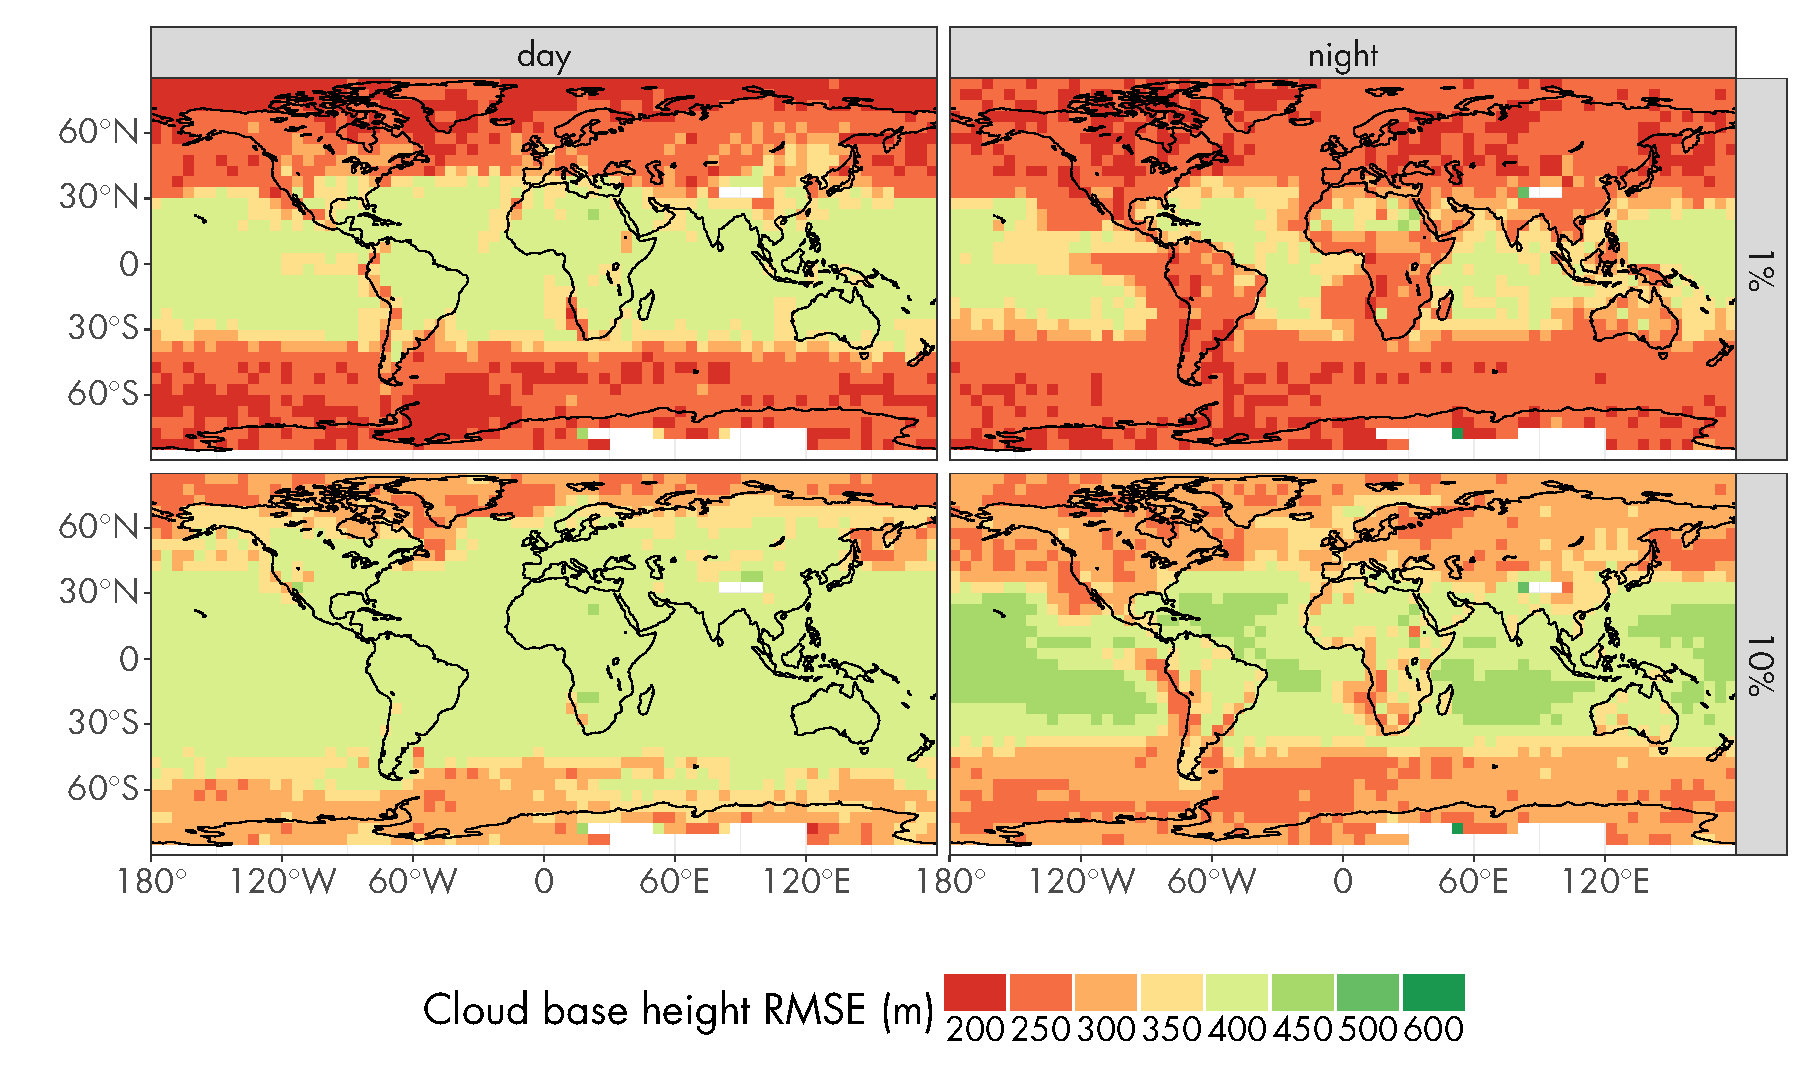
\includegraphics[width=\textwidth]{figure/cfmip-cbase-170926-cbase-uncert-quantiles-1} 

}



\end{knitrout}

        \tcbitem[add to natural height=\myspace, title={Conclusions}]
        \begin{itemize}
        \item CBASE performance is very close to 2B-GEOPROF-LIDAR (which is
          reassuring, since the underlying physical measurement is the same)
        \item The rigorous CBH uncertainty estimate provided by CBASE makes it
          possible to select the lowest-uncertainty cloud bases or to weight
          cloud bases statistically, as appropriate for each analysis
        \item By selecting the lowest-uncertainty cloud bases, the CBH
          uncertainty can be reduced from the 480~m assumed 2B-GEOPROF-LIDAR
          uncertainty to approximately 250~m in the extratropics and
          400~m over tropical oceans
        \item CBASE data will be freely available from the World Data Center
          (Climate) at the German Climate Computing Center
        \end{itemize}
      \end{tcbitemize}
    \end{tcbitemize}
  \end{tcolorbox}
\end{frame}



\end{document}

